\documentclass{extbook}[14pt]
\usepackage{multicol, enumerate, enumitem, hyperref, color, soul, setspace, parskip, fancyhdr, amssymb, amsthm, amsmath, latexsym, units, mathtools}
\everymath{\displaystyle}
\usepackage[headsep=0.5cm,headheight=0cm, left=1 in,right= 1 in,top= 1 in,bottom= 1 in]{geometry}
\usepackage{dashrule}  % Package to use the command below to create lines between items
\newcommand{\litem}[1]{\item #1

\rule{\textwidth}{0.4pt}}
\pagestyle{fancy}
\lhead{}
\chead{Answer Key for Progress Quiz 6 Version B}
\rhead{}
\lfoot{1430-1829}
\cfoot{}
\rfoot{test}
\begin{document}
\textbf{This key should allow you to understand why you choose the option you did (beyond just getting a question right or wrong). \href{https://xronos.clas.ufl.edu/mac1105spring2020/courseDescriptionAndMisc/Exams/LearningFromResults}{More instructions on how to use this key can be found here}.}

\textbf{If you have a suggestion to make the keys better, \href{https://forms.gle/CZkbZmPbC9XALEE88}{please fill out the short survey here}.}

\textit{Note: This key is auto-generated and may contain issues and/or errors. The keys are reviewed after each exam to ensure grading is done accurately. If there are issues (like duplicate options), they are noted in the offline gradebook. The keys are a work-in-progress to give students as many resources to improve as possible.}

\rule{\textwidth}{0.4pt}

\begin{enumerate}\litem{
Determine the domain of the function below.
\[ f(x) = \frac{3}{15x^{2} -12 x -36} \]The solution is \( \text{All Real numbers except } x = -1.200 \text{ and } x = 2.000. \), which is option E.\begin{enumerate}[label=\Alph*.]
\item \( \text{All Real numbers except } x = a, \text{ where } a \in [-3.2, 0.8] \)

All Real numbers except $x = -1.200$, which corresponds to removing only 1 value from the denominator.
\item \( \text{All Real numbers except } x = a, \text{ where } a \in [-32, -28] \)

All Real numbers except $x = -30.000$, which corresponds to removing a distractor value from the denominator.
\item \( \text{All Real numbers.} \)

This corresponds to thinking the denominator has complex roots or that rational functions have a domain of all Real numbers.
\item \( \text{All Real numbers except } x = a \text{ and } x = b, \text{ where } a \in [-32, -28] \text{ and } b \in [17, 19] \)

All Real numbers except $x = -30.000$ and $x = 18.000$, which corresponds to not factoring the denominator correctly.
\item \( \text{All Real numbers except } x = a \text{ and } x = b, \text{ where } a \in [-3.2, 0.8] \text{ and } b \in [2, 5] \)

All Real numbers except $x = -1.200$ and $x = 2.000$, which is the correct option.
\end{enumerate}

\textbf{General Comment:} Recall that dividing by zero is not a real number. Therefore the domain is all real numbers \textbf{except} those that make the denominator 0.
}
\litem{
Solve the rational equation below. Then, choose the interval(s) that the solution(s) belongs to.
\[ \frac{-2}{-7x + 2} + 3 = \frac{-4}{28x -8} \]The solution is \( x = 0.143 \), which is option D.\begin{enumerate}[label=\Alph*.]
\item \( \text{All solutions lead to invalid or complex values in the equation.} \)

This corresponds to thinking $x = 0.143$ leads to dividing by zero in the original equation, which it does not.
\item \( x \in [-0.6,-0.2] \)

$x = -0.429$, which corresponds to not distributing the factor $-7x + 2$ correctly when trying to eliminate the fraction.
\item \( x_1 \in [-0.1, 1.3] \text{ and } x_2 \in [0.37,0.53] \)

$x = 0.143 \text{ and } x = 0.381$, which corresponds to getting the correct solution and believing there should be a second solution to the equation.
\item \( x \in [0.14,3.14] \)

* $x = 0.143$, which is the correct option.
\item \( x_1 \in [-0.6, -0.2] \text{ and } x_2 \in [0.1,0.23] \)

$x = -0.429 \text{ and } x = 0.143$, which corresponds to getting the correct solution and believing there should be a second solution to the equation.
\end{enumerate}

\textbf{General Comment:} Distractors are different based on the number of solutions. Remember that after solving, we need to make sure our solution does not make the original equation divide by zero!
}
\litem{
Solve the rational equation below. Then, choose the interval(s) that the solution(s) belongs to.
\[ \frac{-3x + 0}{-5x + 6} + \frac{-2x^{2} +0 x + 0}{-10x^{2} +22 x -12} = \frac{7}{2x -2} \]The solution is \( \text{There are two solutions: } x = 1.415 \text{ and } x = 3.710 \), which is option B.\begin{enumerate}[label=\Alph*.]
\item \( x \in [3.58,4.52] \)


\item \( x_1 \in [1.34, 2.52] \text{ and } x_2 \in [1.5,4] \)

* $x = 1.415 \text{ and } x = 3.710$, which is the correct option.
\item \( \text{All solutions lead to invalid or complex values in the equation.} \)


\item \( x \in [0.37,1.36] \)


\item \( x_1 \in [1.34, 2.52] \text{ and } x_2 \in [-1.7,2.1] \)


\end{enumerate}

\textbf{General Comment:} Distractors are different based on the number of solutions. Remember that after solving, we need to make sure our solution does not make the original equation divide by zero!
}
\litem{
Determine the domain of the function below.
\[ f(x) = \frac{3}{30x^{2} -43 x + 15} \]The solution is \( \text{All Real numbers except } x = 0.600 \text{ and } x = 0.833. \), which is option B.\begin{enumerate}[label=\Alph*.]
\item \( \text{All Real numbers except } x = a, \text{ where } a \in [14.7, 15.08] \)

All Real numbers except $x = 15.000$, which corresponds to removing a distractor value from the denominator.
\item \( \text{All Real numbers except } x = a \text{ and } x = b, \text{ where } a \in [0.1, 0.79] \text{ and } b \in [0.67, 1.24] \)

All Real numbers except $x = 0.600$ and $x = 0.833$, which is the correct option.
\item \( \text{All Real numbers except } x = a, \text{ where } a \in [0.1, 0.79] \)

All Real numbers except $x = 0.600$, which corresponds to removing only 1 value from the denominator.
\item \( \text{All Real numbers.} \)

This corresponds to thinking the denominator has complex roots or that rational functions have a domain of all Real numbers.
\item \( \text{All Real numbers except } x = a \text{ and } x = b, \text{ where } a \in [14.7, 15.08] \text{ and } b \in [29.71, 30.12] \)

All Real numbers except $x = 15.000$ and $x = 30.000$, which corresponds to not factoring the denominator correctly.
\end{enumerate}

\textbf{General Comment:} Recall that dividing by zero is not a real number. Therefore the domain is all real numbers \textbf{except} those that make the denominator 0.
}
\litem{
Choose the equation of the function graphed below.

\begin{center}
    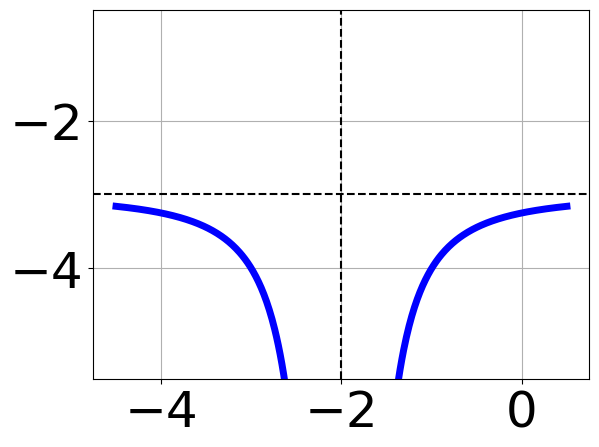
\includegraphics[width=0.5\textwidth]{../Figures/rationalGraphToEquationCopyB.png}
\end{center}


The solution is \( f(x) = \frac{-1}{(x - 3)^2} - 3 \), which is option B.\begin{enumerate}[label=\Alph*.]
\item \( f(x) = \frac{1}{x + 3} - 3 \)

Corresponds to thinking the graph was a shifted version of $\frac{1}{x}$, using the general form $f(x) = \frac{a}{(x+h)^2}+k$, and the opposite leading coefficient.
\item \( f(x) = \frac{-1}{(x - 3)^2} - 3 \)

This is the correct option.
\item \( f(x) = \frac{1}{(x + 3)^2} - 3 \)

Corresponds to using the general form $f(x) = \frac{a}{(x+h)^2}+k$ and the opposite leading coefficient.
\item \( f(x) = \frac{-1}{x - 3} - 3 \)

Corresponds to thinking the graph was a shifted version of $\frac{1}{x}$.
\item \( \text{None of the above} \)

This corresponds to believing the vertex of the graph was not correct.
\end{enumerate}

\textbf{General Comment:} Remember that the general form of a basic rational equation is $ f(x) = \frac{a}{(x-h)^n} + k$, where $a$ is the leading coefficient (and in this case, we assume is either $1$ or $-1$), $n$ is the degree (in this case, either $1$ or $2$), and $(h, k)$ is the intersection of the asymptotes.
}
\litem{
Choose the graph of the equation below.
\[ f(x) = \frac{1}{(x + 3)^2} - 3 \]The solution is the graph below, which is option E.
\begin{center}
    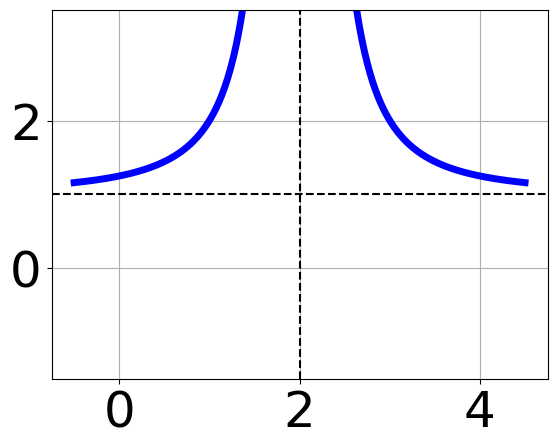
\includegraphics[width=0.3\textwidth]{../Figures/rationalEquationToGraphEB.png}
\end{center}\begin{enumerate}[label=\Alph*.]
\begin{multicols}{2}
\item 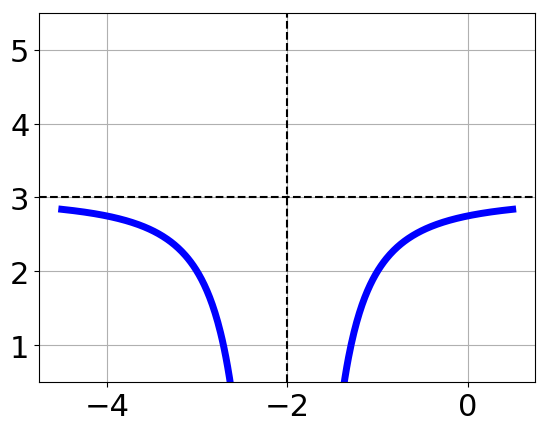
\includegraphics[width = 0.3\textwidth]{../Figures/rationalEquationToGraphAB.png}
\item 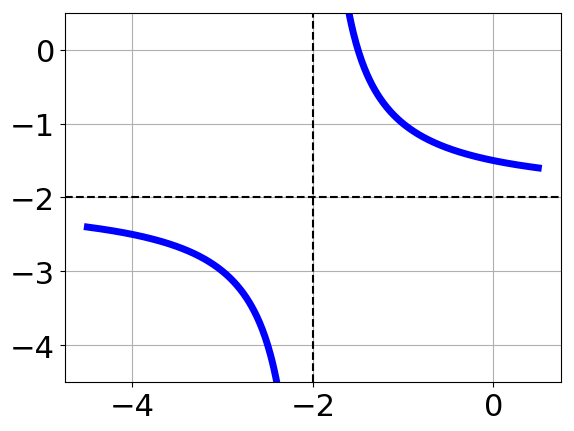
\includegraphics[width = 0.3\textwidth]{../Figures/rationalEquationToGraphBB.png}
\item 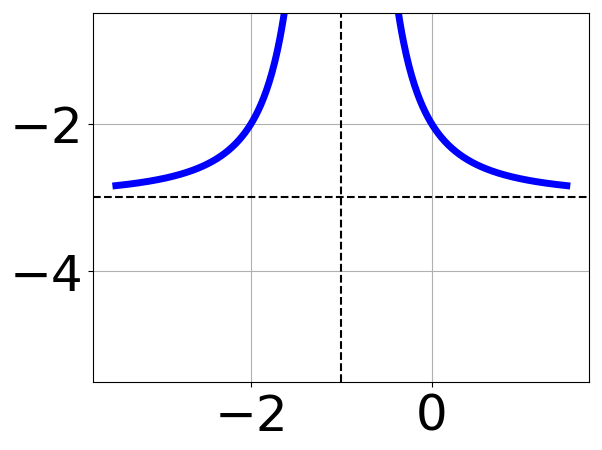
\includegraphics[width = 0.3\textwidth]{../Figures/rationalEquationToGraphCB.png}
\item 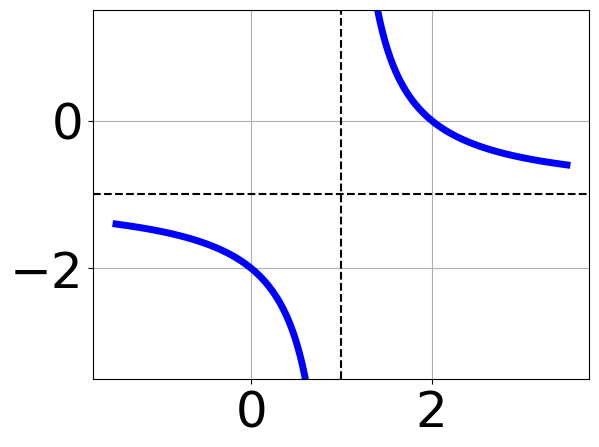
\includegraphics[width = 0.3\textwidth]{../Figures/rationalEquationToGraphDB.png}
\end{multicols}\item None of the above.\end{enumerate}
\textbf{General Comment:} Remember that the general form of a basic rational equation is $ f(x) = \frac{a}{(x-h)^n} + k$, where $a$ is the leading coefficient (and in this case, we assume is either $1$ or $-1$), $n$ is the degree (in this case, either $1$ or $2$), and $(h, k)$ is the intersection of the asymptotes.
}
\litem{
Solve the rational equation below. Then, choose the interval(s) that the solution(s) belongs to.
\[ \frac{-27}{-45x -81} + 1 = \frac{-27}{-45x -81} \]The solution is \( \text{all solutions are invalid or lead to complex values in the equation.} \), which is option D.\begin{enumerate}[label=\Alph*.]
\item \( x_1 \in [-4.8, -0.8] \text{ and } x_2 \in [-4.8,-0.8] \)

$x = -1.800 \text{ and } x = -1.800$, which corresponds to getting the correct solution and believing there should be a second solution to the equation.
\item \( x_1 \in [-4.8, -0.8] \text{ and } x_2 \in [0.8,2.8] \)

$x = -1.800 \text{ and } x = 1.800$, which corresponds to getting the correct solution and believing there should be a second solution to the equation.
\item \( x \in [-2.8,-0.8] \)

$x = -1.800$, which corresponds to not checking if this value leads to dividing by 0 in the original equation and thus is not a valid solution.
\item \( \text{All solutions lead to invalid or complex values in the equation.} \)

*$x = -1.800$ leads to dividing by 0 in the original equation and thus is not a valid solution, which is the correct option.
\item \( x \in [1.8,3.8] \)

$x = 1.800$, which corresponds to not distributing the factor $-45x -81$ correctly when trying to eliminate the fraction.
\end{enumerate}

\textbf{General Comment:} Distractors are different based on the number of solutions. Remember that after solving, we need to make sure our solution does not make the original equation divide by zero!
}
\litem{
Choose the graph of the equation below.
\[ f(x) = \frac{-1}{x + 3} + 1 \]The solution is the graph below, which is option E.
\begin{center}
    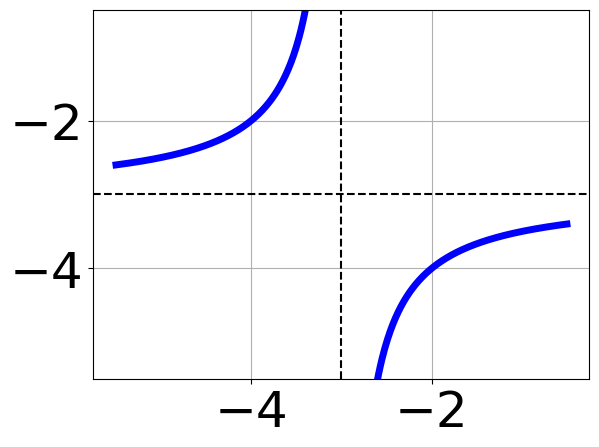
\includegraphics[width=0.3\textwidth]{../Figures/rationalEquationToGraphCopyEB.png}
\end{center}\begin{enumerate}[label=\Alph*.]
\begin{multicols}{2}
\item 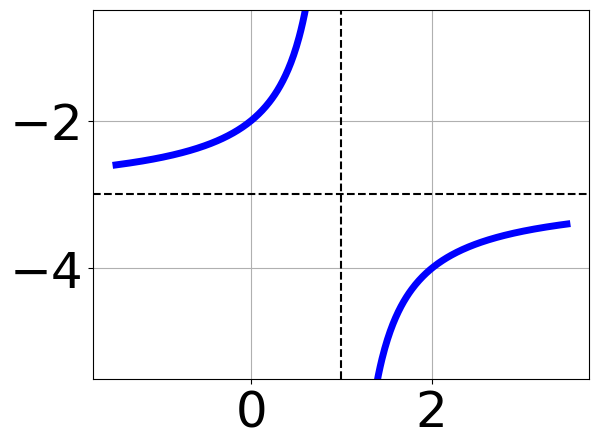
\includegraphics[width = 0.3\textwidth]{../Figures/rationalEquationToGraphCopyAB.png}
\item 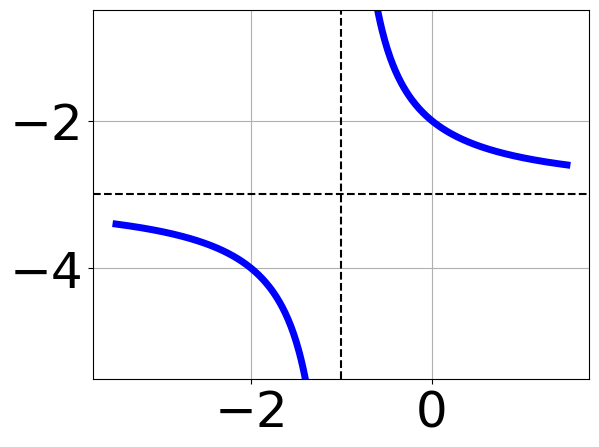
\includegraphics[width = 0.3\textwidth]{../Figures/rationalEquationToGraphCopyBB.png}
\item 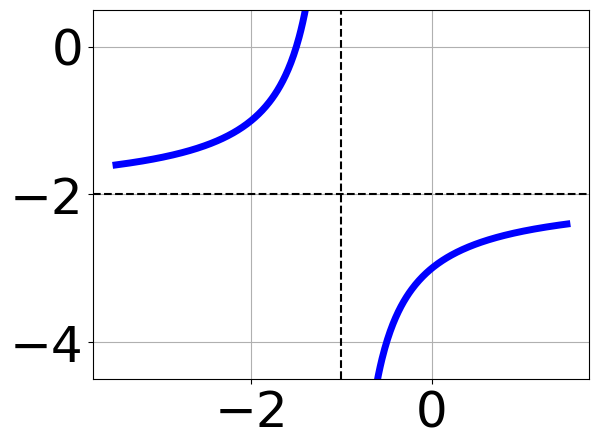
\includegraphics[width = 0.3\textwidth]{../Figures/rationalEquationToGraphCopyCB.png}
\item 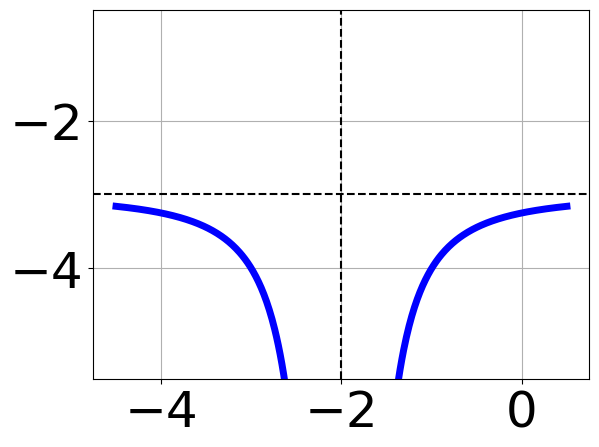
\includegraphics[width = 0.3\textwidth]{../Figures/rationalEquationToGraphCopyDB.png}
\end{multicols}\item None of the above.\end{enumerate}
\textbf{General Comment:} Remember that the general form of a basic rational equation is $ f(x) = \frac{a}{(x-h)^n} + k$, where $a$ is the leading coefficient (and in this case, we assume is either $1$ or $-1$), $n$ is the degree (in this case, either $1$ or $2$), and $(h, k)$ is the intersection of the asymptotes.
}
\litem{
Choose the equation of the function graphed below.

\begin{center}
    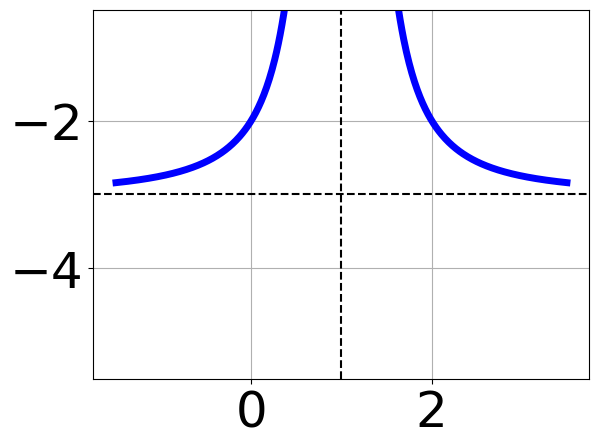
\includegraphics[width=0.5\textwidth]{../Figures/rationalGraphToEquationB.png}
\end{center}


The solution is \( f(x) = \frac{1}{(x - 3)^2} - 3 \), which is option C.\begin{enumerate}[label=\Alph*.]
\item \( f(x) = \frac{1}{x - 3} - 3 \)

Corresponds to thinking the graph was a shifted version of $\frac{1}{x}$.
\item \( f(x) = \frac{-1}{x + 3} - 3 \)

Corresponds to thinking the graph was a shifted version of $\frac{1}{x}$, using the general form $f(x) = \frac{a}{(x+h)^2}+k$, and the opposite leading coefficient.
\item \( f(x) = \frac{1}{(x - 3)^2} - 3 \)

This is the correct option.
\item \( f(x) = \frac{-1}{(x + 3)^2} - 3 \)

Corresponds to using the general form $f(x) = \frac{a}{(x+h)^2}+k$ and the opposite leading coefficient.
\item \( \text{None of the above} \)

This corresponds to believing the vertex of the graph was not correct.
\end{enumerate}

\textbf{General Comment:} Remember that the general form of a basic rational equation is $ f(x) = \frac{a}{(x-h)^n} + k$, where $a$ is the leading coefficient (and in this case, we assume is either $1$ or $-1$), $n$ is the degree (in this case, either $1$ or $2$), and $(h, k)$ is the intersection of the asymptotes.
}
\litem{
Solve the rational equation below. Then, choose the interval(s) that the solution(s) belongs to.
\[ \frac{4x + 0}{7x + 2} + \frac{-5x^{2} +0 x + 0}{42x^{2} +26 x + 4} = \frac{2}{6x + 2} \]The solution is \( \text{There are two solutions: } x = -0.327 \text{ and } x = 0.643 \), which is option E.\begin{enumerate}[label=\Alph*.]
\item \( x \in [-0.34,-0.33] \)


\item \( x_1 \in [-0.33, -0.32] \text{ and } x_2 \in [-0.59,0.1] \)


\item \( x \in [0.64,0.65] \)


\item \( \text{All solutions lead to invalid or complex values in the equation.} \)


\item \( x_1 \in [-0.33, -0.32] \text{ and } x_2 \in [0.36,1.05] \)

* $x = -0.327 \text{ and } x = 0.643$, which is the correct option.
\end{enumerate}

\textbf{General Comment:} Distractors are different based on the number of solutions. Remember that after solving, we need to make sure our solution does not make the original equation divide by zero!
}
\end{enumerate}

\end{document}